\chapter{M2Go Part 1: C\&M Org}
\label{cha:cm_org}

\section{Exercise OnboardingCompletion}
This section contains the answers to the questions of the exercise "OnboardingCompletion". 
The first section describes the author's motivation for choosing this module. 
The second section, the description of the timesheet, explains the author's understanding of the time sheet and its importance.

\subsection{Write an Introduction}
While working as a student intern at Capgemini, I had the opportunity to work in web development for six months.
During this time, I was an integral part of a dynamic team dedicated to an internal project focused on managing events and training programs for their employees.
It was during this time that I discovered the importance of web development and found myself genuinely passionate about the subject.

This exposure gave me a fundamental understanding of web development's potential.
I am thrilled to have chosen this specific module for further education. 
Furthermore, I am eager to explore the possibilities web development offers and look forward to the next few months.

\begin{figure}[H]
    \centering
    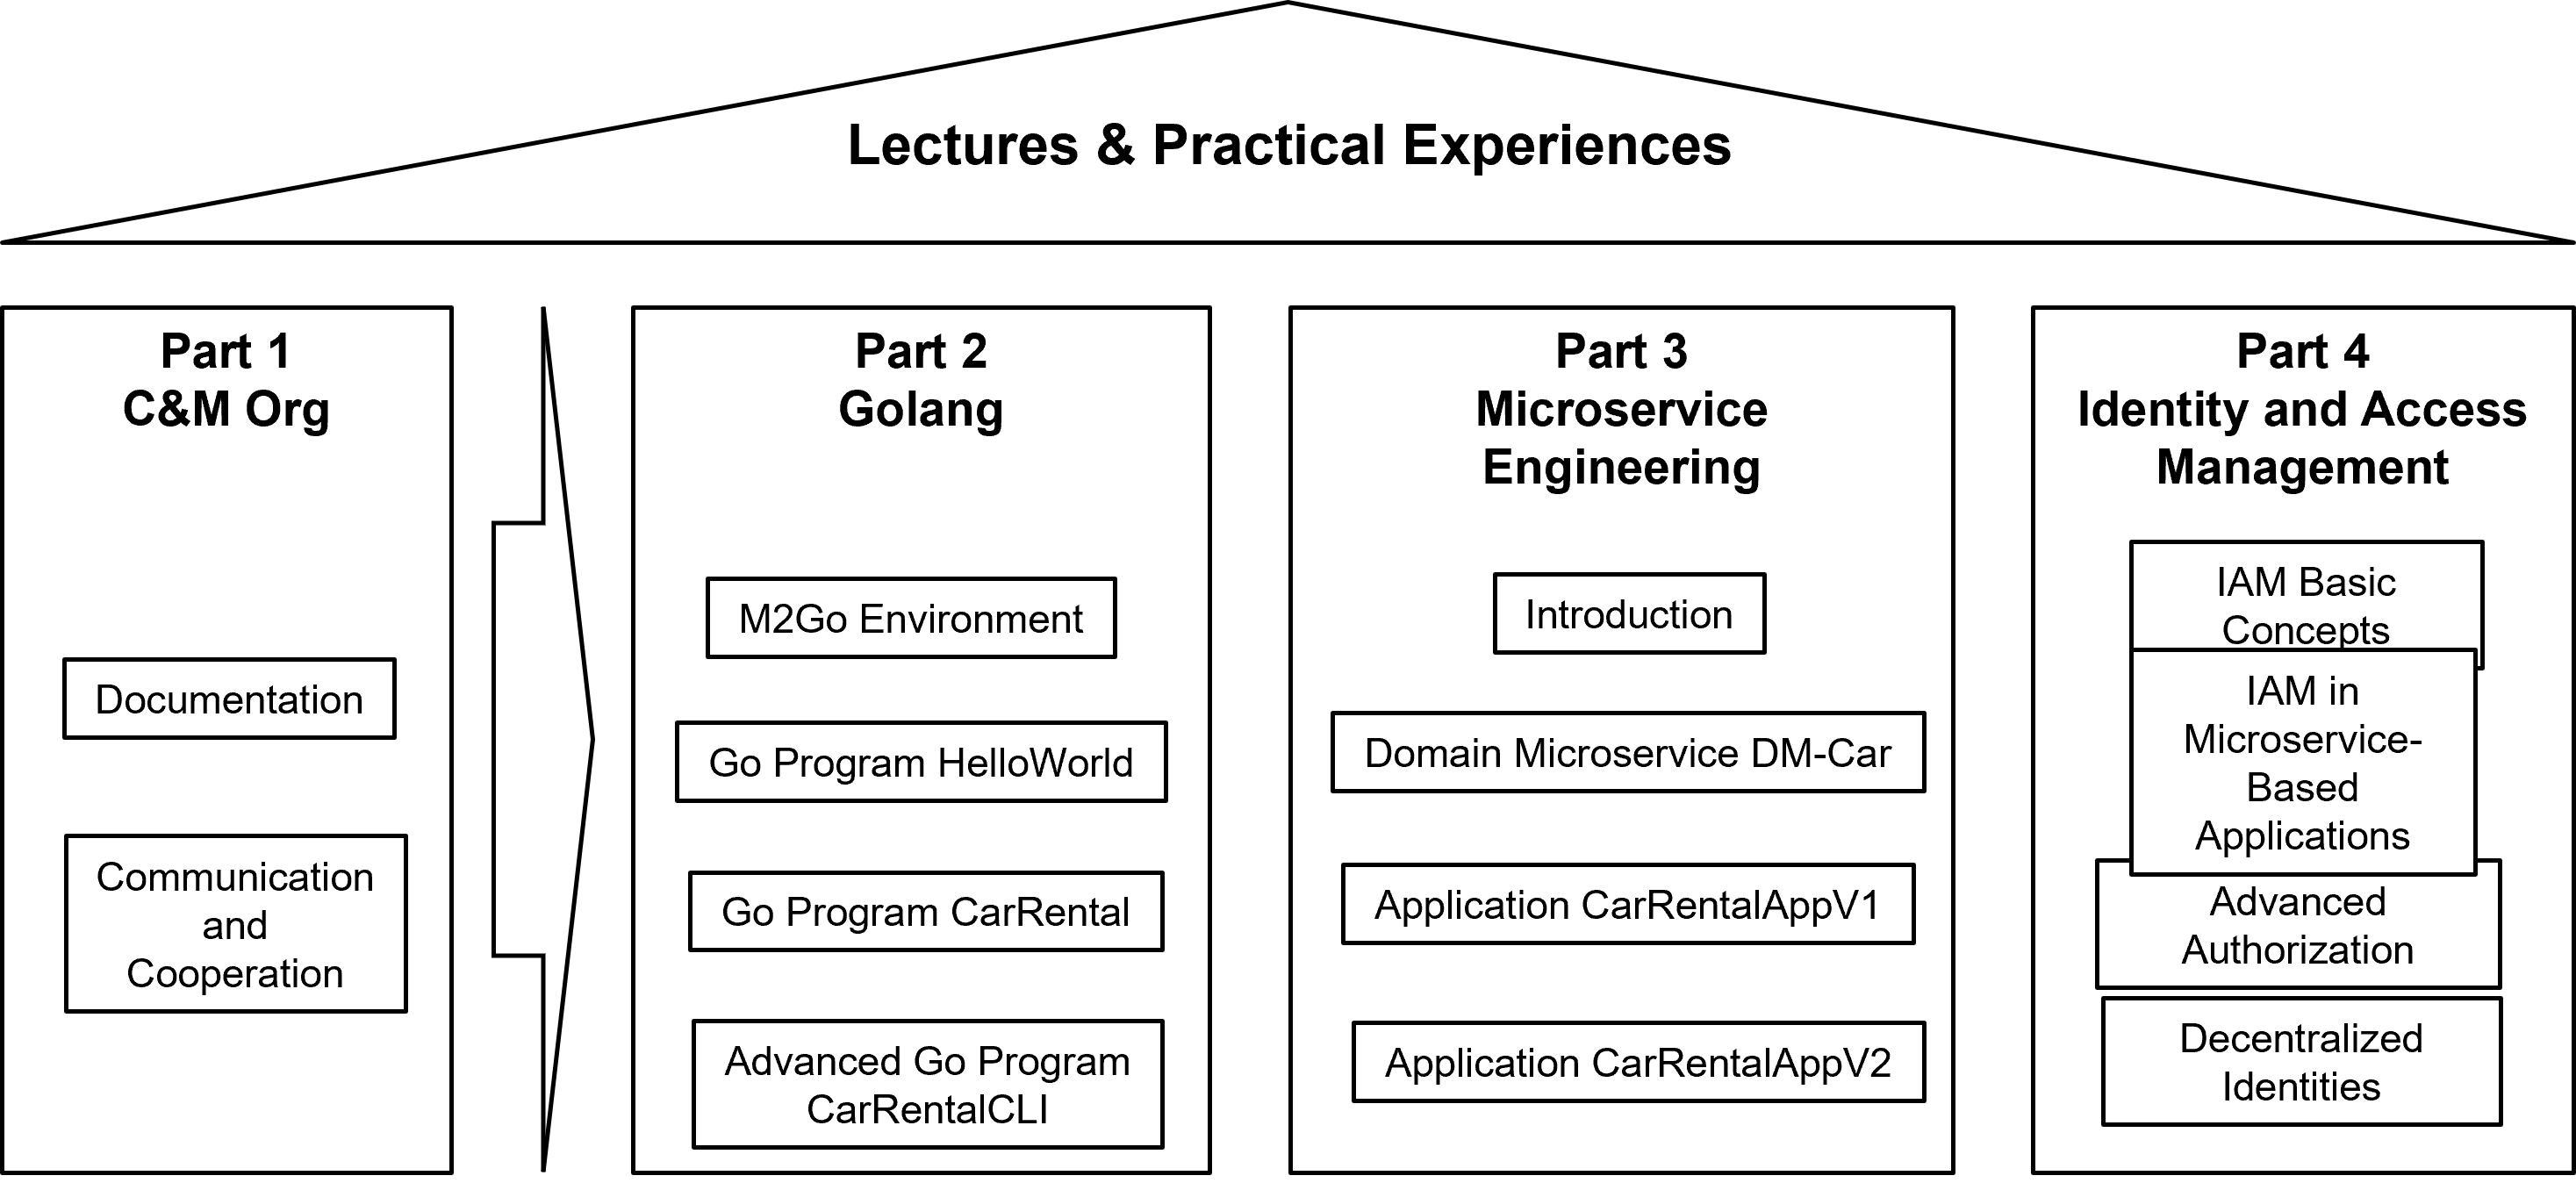
\includegraphics[width=0.8\textwidth]{figures/onboarding/m2go_parts.png}
    \caption{M2Go Parts}
    \label{fig:m2go_parts}
\end{figure}

\subsection{Describe the Time Sheet}
The time sheet offers a certain overview of the time spent on the project. 
Furthermore, one can compare themselves to the set standards of the project, therefore enabling better time management.
After understanding the provided interface, I was able to fill out the timesheet without any problems.

It helps me and my colleagues build a more structured daily routine and therefore increase productivity. Possible roadblocks or challenges can be identified and solved more easily.
Also, it helps the project manager to keep track of the progress and to identify possible problems, maybe assist if needed.

In essence, the timesheet contributes to streamlined project management and increased, more structured productivity for both individual contributors and project leaders.

\begin{figure}[h]
    \centering
    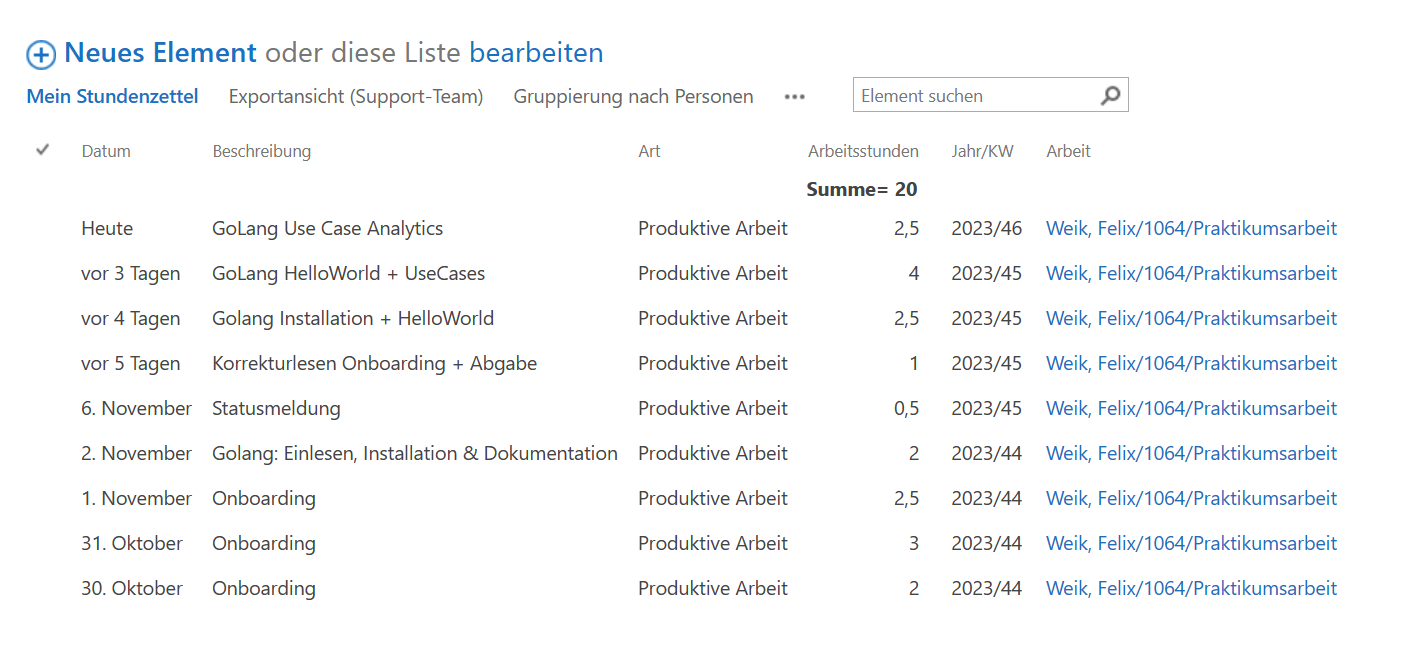
\includegraphics[width=0.9\textwidth]{figures/onboarding/stundenzettel_screendump.png}
    \caption{Screendump of the time sheet}
    \label{fig:time_sheet}
\end{figure}
